%% Los capitulos inician con \chapter{T'itulo}, estos aparecen numerados y
%% se incluyen en el 'indice general.
%%
%% Recuerda que aqu'i ya puedes escribir acentos como: 'a, 'e, 'i, etc.
%% La letra n con tilde es: 'n.

\chapter{Análisis, Planificación y Diseño del Sistema}

En este capítulo se explican los procesos que fueron necesarios para la investigación y creación del sistema para inferir la deserción de clientes. Esta es la fase inicial donde se analizan los objetivos del proyecto y se definen las lineas de diseño base para la creación del sistema.

\section{Análisis y Definición del Modelo}

Como se describió anteriormente, el ámbito no contractual y continuo en el que se desarrolla el comercio electrónico, es el más común pero el mas desafiante a la hora de evaluar, analizar y obtener información de valor para los negocios. 

	Inicialmente se evaluó la posibilidad de utilizar técnicas de inteligencia artificial o aprendizaje automático, pero debido al escenario en el que se esta trabajando, donde la deserción del cliente no es explícitamente observable y puede ocurrir en cualquier momento, se dificulta diferenciar entre los clientes que se han ido indefinidamente y los que volverán en el futuro, además, la naturaleza y escasez de datos de acceso público, no permite entrenar un modelo complejo que pudiese predecir ese comportamiento.

	Dicho esto, se buscó una solución mediante uno o varios modelos estadísticos. Este tipo de enfoque es considerado efectivo para este ámbito, ya que se pueden generar ecuaciones predeterminadas que se adapten a los datos obtenidos, inferir la relación que existe entre las variables y así generar valores esperados.

	Luego de decidir el enfoque de la solución, se comenzó una investigación exhaustiva para determinar que variables modelar y que relaciones evaluar. Este problema ya se ha atacado antes, en el articulo Counting Your Customers: Who Are They and What Will They Do Next? \cite{schmittlein1987} se plantea una solución que se basa en predecir el numero de transacciones de un cliente en el futuro, si bien los resultados de este modelo son efectivos, existe un problema de implementación desde el punto de vista computacional debido a la complejidad de las funciones matemáticas utilizadas en el modelo.

	En el artículo “Counting Your Customers” the Easy Way: An Alternative to the Pareto/NBD Model \cite{fader2005}, los autores realizaron una mejora considerable al modelo Pareto / NBD, simplificando así su implementación y manteniendo los resultados.

	Posteriormente, en una nota A Step-by-Step Derivation of the BG/NBD Model \cite{fader2019}, los autores describieron los pasos para derivar los resultados obtenidos anteriormente, lo que permitió la implementación del modelo en código Python por parte de Cameron Davidson-Pilon, creando así la biblioteca Lifetimes que será el pilar base del sistema para predecir la deserción de clientes en un e-commerce.

\section{Arquitectura del Sistema}

La solución al problema planteado consta de un sistema donde se integran tres módulos: el modelo, la API y la aplicación web (Figura). El módulo de modelo se encarga de procesar la data que se obtuvo y generar un modelo estadístico para la predicción de la tasa de deserción de los clientes. Este proceso se realiza una vez, es decir, no es necesario crear otro modelo o ajustar el modelo actual con los datos ingresados por un usuario mediante la interfaz.

\begin{figure}[H]
	\centering 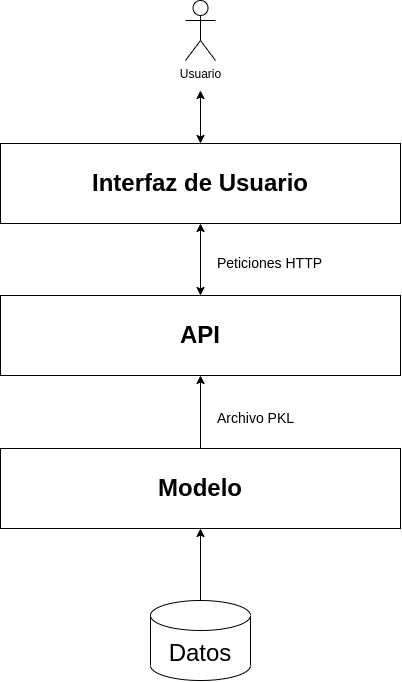
\includegraphics[width=0.50\textwidth]{images/arquitectura-proyecto-de-grado.png}
	\caption{Arquitectura del Sistema}
	\label{fig:arq}
\end{figure}

	La API sirve de middleware o capa intermedia entre el modelo y la interfaz del usuario, es decir, esta se encargaría de recibir los datos de la aplicación web, procesarlos haciendo uso del modelo y devolver el resultado de nuevo a la interfaz para que el usuario pueda verlos.

	Finalmente, la interfaz tiene como finalidad permitir introducir al usuario al sistema, recibir su entrada como una lista de transacciones que están representadas por una fecha y un identificador de cliente, enviar esa información a la API para ser procesada, recibir el resultado y mostrarle un gráfico de probabilidad por cada cliente donde se exprese la probabilidad de que este haya desertado en un punto en el tiempo futuro.
	
	La comunicación entre el módulo del modelo y la API se realizaría mediante un archivo PKL que contiene los parámetros del modelo creado, el cual será importado por la API al momento de su ejecución y utilizado para generar predicciones. La API y la aplicación web hablarían mediante peticiones HTTP e intercambiarían la información en formato JSON.

\section{Requerimientos}

A pesar de que la metodología de desarrollo es ágil, se consideró importante definir una serie de requerimientos como base que debe cumplir el sistema, esto con la finalidad de mantener un enfoque durante la implementación y que las tareas del backlog tengan un objetivo en común.

	Acorde a lo descrito en la sección anterior en la cual se desarrolló una arquitectura para el sistema, la lista de requerimientos por módulo que se estableció es la siguiente: 

\subsection{Modelo}

\subsubsection{Requerimientos Funcionales}

\begin{itemize}
	\item El sistema genera un modelo estadístico que pueda predecir la deserción de clientes de un e-commerce.
\end{itemize}

\subsubsection{Requerimientos no Funcionales}

\begin{itemize}
	\item Se debe importar las transacciones de un archivo CSV.
	\item Se debe procesar la data en un dataframe con las características definidas por la biblioteca lifetimes.
	\item El modelo se debe guardar en un archivo con formato PKL en la carpeta del módulo API.
	\item El código fuente del modelo debe estar disponible dentro del repositorio del proyecto en GitHub.
	\item Se debe implementar el modelo en un Jupyter Notebook.
	\item En el Jupyter Notebook debe estar expresado el proceso de generación del modelo.
	\item Se deben mostrar ejemplos de uso del modelo.
\end{itemize}

\subsection{API}

\subsubsection{Requerimientos Funcionales}

\begin{itemize}
	\item Crear una ruta (/conditional-probability-alive) donde se reciba una lista de transacciones por usuario y se retorne la probabilidad de vida de cada cliente en 500 unidades de tiempo desde la primera transacción.
\end{itemize}

\subsubsection{Requerimientos no Funcionales}

\begin{itemize}
	\item La API será usada por una aplicación web.
	\item La API usará la arquitectura REST.
	\item El formato de entrada y salida debe estar descrito en el archivo README.md correspondiente a la carpeta del proyecto.
	\item Las instrucciones de ejecución deben estar contempladas en el archivo README.md correspondiente a la carpeta del proyecto.
	\item El formato debe especificar en cada campo con su clave y tipo de dato aceptado.
	\item Permitir el acceso libre a la API.
	\item La API debe procesar y retornar datos en formato JSON.
	\item La API debe estar disponible de manera pública mediante un enlace de prueba.
	\item El código fuente de la API debe estar disponible dentro del repositorio del proyecto en GitHub.
\end{itemize}

\subsection{Aplicación Web}

\subsubsection{Requerimientos Funcionales}

\begin{itemize}
	\item El usuario ingresa la lista de transacciones de los clientes y obtiene la probabilidad de que los clientes desertara de su negocio en un grafico lineal.
\end{itemize}

\subsubsection{Requerimientos no Funcionales}

\begin{itemize}
	\item Se debe validar que las fechas ingresadas por el usuario sigan el formato DD-MM-AAAA.
	\item No se pueden ingresar o enviar transacciones sin fecha o identificador de cliente.
	\item El identificador de cliente es una cadena de caracteres con tamaño mayor de tres.
	\item Las instrucciones de ejecución deben estar contempladas en el archivo README.md correspondiente a la carpeta del proyecto.
	\item Se debe describir brevemente las instrucciones de uso en el archivo README.md correspondiente a la carpeta del proyecto.
	\item La aplicación web debe procesar y retornar datos en formato JSON.
	\item Se debe describir brevemente las instrucciones de uso la interfaz.
	\item Se debe acceder a la API mediante un método POST.
	\item El código fuente de la aplicación web debe estar disponible dentro del repositorio del proyecto en GitHub.
\end{itemize}

\section{Diseño de Interfaz de Usuario}

Lo más importante en el sistema es permitir a un usuario ingresar una lista de transacciones de clientes y que este luego pueda ver la probabilidad de que estos clientes deserten, es por ello que se plantea una interfaz simple de una sola página web (ver Figura 2).

\begin{figure}[H]
	\centering 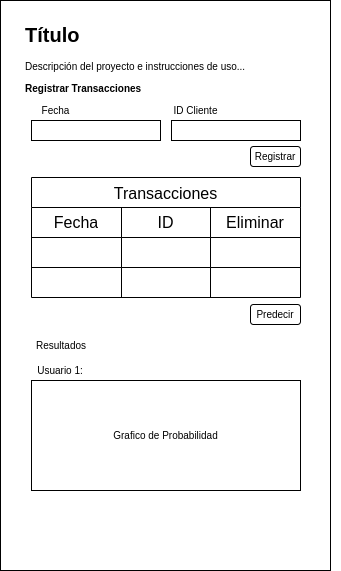
\includegraphics[width=0.50\textwidth]{images/ui.png}
	\caption{Intefaz de Usuario}
	\label{fig:ui}
\end{figure}

La página web inicialmente muestra información sobre el proyecto como título, descripción e instrucciones sobre como utilizar el sistema, luego se muestra un formulario de entrada donde el usuario puede registrar una transacción. La transacción consiste de una fecha en formato DD-MM-AAAA y un identificador de cliente. 

La experiencia de usuario en el sistema es simple, cuando se registra una transacción válida, esta se agrega a una tabla que el usuario puede visualizar con la opción de eliminar alguna transacción ya registrada.

El usuario al terminar de registrar las transacciones hace clic en el botón “predecir”, luego de esto se muestra un gráfico que representa la probabilidad de desertar de un cliente a lo largo del tiempo y comenzando desde la fecha de la primera transacción registrada del cliente. Se construye un gráfico por cada identificador de cliente ingresado.